%%%%%%%%%%%%%%%%%%%%%%%%%%%%%%%%%%%%%%
%%%%%%%%%%%%%%%%%%%%%%%%%%%%%%%%%%%%%%
% Do not edit the TeX file your work
% will be overwritten.  Edit the RnW
% file instead.
%%%%%%%%%%%%%%%%%%%%%%%%%%%%%%%%%%%%%%
%%%%%%%%%%%%%%%%%%%%%%%%%%%%%%%%%%%%%%





\newcommand{\DefineMacros}{
\newcommand{\SimNumObs}{5,000}
\newcommand{\SimTrueTheta}{0.5}
\newcommand{\SimAccNumObs}{5,000}
\newcommand{\SimAccSigx}{2}
\newcommand{\SimAccSigeps}{1}
\newcommand{\SimAccPercentMax}{10}

}

%%%%%%%%%%%%%%%%%%%%%%
%%%%%%%%%%%%%%%%%%%%%%
%%%%%%%%%%%%%%%%%%%%%%
% Tables

\newcommand{\CashTransfersResultsTable}{
% \input{figures/cash_transfers_re_run_table.tex}


\begin{table}\scriptsize 
\begin{tabular}{|ccccc|}
\toprule
Study case & Original estimate  & Target change  & Refit estimate  & Observations dropped \\
\midrule
\midrule
& &  Sign change &  \textbf{-0.656 (3.745)} &  252 = 2.30\%\\
Poor, period 8  &  17.312 (4.576)* &  Significance change &  \textbf{7.284 (4.087)} &  83 = 0.76\%\\
& &  Significant sign change &  \textbf{-7.212 (3.443)*} &  464 = 4.24\%\\
\midrule
& &  Sign change &  \textbf{-1.377 (4.406)} &  345 = 3.58\%\\
Poor, period 9  &  27.924 (5.770)* &  Significance change &  \textbf{7.077 (4.555)} &  146 = 1.52\%\\
& &  Significant sign change &  \textbf{-8.951 (4.251)*} &  588 = 6.11\%\\
\midrule
& &  Sign change &  \textbf{-2.559 (3.541)} &  697 = 6.63\%\\
Poor, period 10  &  33.861 (4.468)* &  Significance change &  \textbf{4.806 (3.684)} &  435 = 4.14\%\\
& &  Significant sign change &  \textbf{-9.416 (3.296)*} &  986 = 9.37\%\\
\midrule
& &  Sign change &  \textbf{0.260 (6.410)} &  5 = 0.11\%\\
Non-poor, period 8  &  -5.444 (7.133) &  Significance change &  -12.845 (6.635) &  16 = 0.35\%\\
& &  Significant sign change &  9.670 (5.573) &  24 = 0.52\%\\
\midrule
& &  Sign change &  \textbf{-0.365 (7.542)} &  21 = 0.55\%\\
Non-poor, period 9  &  22.852 (10.000)* &  Significance change &  \textbf{16.506 (9.114)} &  3 = 0.08\%\\
& &  Significant sign change &  -11.733 (7.113) &  53 = 1.38\%\\
\midrule
& &  Sign change &  \textbf{-0.573 (6.750)} &  30 = 0.70\%\\
Non-poor, period 10  &  21.493 (9.405)* &  Significance change &  \textbf{16.262 (8.927)} &  3 = 0.07\%\\
& &  Significant sign change &  -10.845 (6.467) &  92 = 2.16\%\\
\midrule
\bottomrule
\end{tabular}
\caption{ Cash transfers results for various periods and treatment groups. The ``Refit estimate'' column shows the result of re-fitting the model removing the Approximate Most Influential Set. Stars indicate significance at the 5\% level.  Refits that achieved the desired change are bolded. }
\label{table:cash_transfers_re_run_table}
\end{table}


}

%%%%%%%%%%%%%%%%%%%
% OHIE

\newcommand{\OHIEResultsTable}{
% \input{figures/OHIE_table_9_IV_re_run_table.tex}


\begin{table}\scriptsize 
\begin{tabular}{|ccccc|}
\toprule
Study case & Original estimate  & Target change  & Refit estimate  & Observations dropped \\
\midrule
\midrule
& &  Sign change &  \textbf{-0.006 (0.025)} &  275 = 1.18\%\\
Health genflip 12m  &  0.133 (0.026)* &  Significance change &  \textbf{0.044 (0.026)} &  162 = 0.69\%\\
& &  Significant sign change &  -0.043 (0.024) &  381 = 1.63\%\\
\midrule
& &  Sign change &  \textbf{-0.003 (0.015)} &  155 = 0.66\%\\
Health notpoor 12m  &  0.099 (0.018)* &  Significance change &  \textbf{0.027 (0.016)} &  100 = 0.43\%\\
& &  Significant sign change &  \textbf{-0.030 (0.015)*} &  219 = 0.94\%\\
\midrule
& &  Sign change &  \textbf{-0.006 (0.022)} &  197 = 0.84\%\\
Health change flip 12m  &  0.113 (0.023)* &  Significance change &  \textbf{0.039 (0.022)} &  106 = 0.45\%\\
& &  Significant sign change &  \textbf{-0.049 (0.022)*} &  291 = 1.24\%\\
\midrule
& &  Sign change &  \textbf{-0.023 (0.535)} &  73 = 0.33\%\\
Not bad days total 12m  &  1.317 (0.563)* &  Significance change &  \textbf{1.078 (0.558)} &  10 = 0.05\%\\
& &  Significant sign change &  -1.009 (0.521) &  144 = 0.66\%\\
\midrule
& &  Sign change &  \textbf{-0.040 (0.577)} &  87 = 0.41\%\\
Not bad days physical 12m  &  1.585 (0.606)* &  Significance change &  \textbf{1.131 (0.597)} &  20 = 0.09\%\\
& &  Significant sign change &  \textbf{-1.141 (0.566)*} &  164 = 0.77\%\\
\midrule
& &  Sign change &  \textbf{-0.062 (0.607)} &  123 = 0.57\%\\
Not bad days mental 12m  &  2.082 (0.640)* &  Significance change &  \textbf{1.171 (0.625)} &  42 = 0.19\%\\
& &  Significant sign change &  \textbf{-1.201 (0.594)*} &  212 = 0.98\%\\
\midrule
& &  Sign change &  \textbf{-0.005 (0.024)} &  123 = 0.53\%\\
Nodep Screen 12m  &  0.078 (0.025)* &  Significance change &  \textbf{0.046 (0.024)} &  42 = 0.18\%\\
& &  Significant sign change &  \textbf{-0.050 (0.023)*} &  220 = 0.95\%\\
\midrule
\bottomrule
\end{tabular}
\caption{ Medicaid profit results with IV for a range of outcome variables.  The ``Refit estimate'' column shows the result of re-fitting the model removing the Approximate Most Influential Set. Stars indicate significance at the 5\% level.  Refits that achieved the desired change are bolded. }
\label{table:ohie_profit_results_iv}
\end{table}



\begin{table}\scriptsize 
\begin{tabular}{|ccccc|}
\toprule
Study case & Original estimate  & Target change  & Refit estimate  & Observations dropped \\
\midrule
\midrule
& &  Sign change &  \textbf{-0.004 (0.008)} &  286 = 1.22\%\\
Health genflip 12m  &  0.039 (0.008)* &  Significance change &  \textbf{0.013 (0.008)} &  163 = 0.70\%\\
& &  Significant sign change &  \textbf{-0.021 (0.008)*} &  422 = 1.81\%\\
\midrule
& &  Sign change &  \textbf{-0.001 (0.005)} &  156 = 0.67\%\\
Health notpoor 12m  &  0.029 (0.005)* &  Significance change &  \textbf{0.008 (0.005)} &  101 = 0.43\%\\
& &  Significant sign change &  \textbf{-0.009 (0.004)*} &  224 = 0.96\%\\
\midrule
& &  Sign change &  \textbf{-0.002 (0.006)} &  198 = 0.85\%\\
Health change flip 12m  &  0.033 (0.007)* &  Significance change &  \textbf{0.011 (0.007)} &  106 = 0.45\%\\
& &  Significant sign change &  \textbf{-0.015 (0.006)*} &  292 = 1.25\%\\
\midrule
& &  Sign change &  \textbf{-0.013 (0.157)} &  74 = 0.34\%\\
Not bad days total 12m  &  0.381 (0.162)* &  Significance change &  \textbf{0.306 (0.161)} &  11 = 0.05\%\\
& &  Significant sign change &  \textbf{-0.309 (0.153)*} &  147 = 0.67\%\\
\midrule
& &  Sign change &  \textbf{-0.017 (0.169)} &  88 = 0.41\%\\
Not bad days physical 12m  &  0.459 (0.175)* &  Significance change &  \textbf{0.328 (0.172)} &  20 = 0.09\%\\
& &  Significant sign change &  \textbf{-0.344 (0.165)*} &  166 = 0.78\%\\
\midrule
& &  Sign change &  \textbf{-0.027 (0.178)} &  124 = 0.57\%\\
Not bad days mental 12m  &  0.603 (0.184)* &  Significance change &  \textbf{0.340 (0.181)} &  42 = 0.19\%\\
& &  Significant sign change &  \textbf{-0.381 (0.175)*} &  216 = 1.00\%\\
\midrule
& &  Sign change &  \textbf{-0.001 (0.007)} &  123 = 0.53\%\\
Nodep Screen 12m  &  0.023 (0.007)* &  Significance change &  \textbf{0.013 (0.007)} &  43 = 0.19\%\\
& &  Significant sign change &  \textbf{-0.015 (0.007)*} &  225 = 0.97\%\\
\midrule
\bottomrule
\end{tabular}
\caption{ Medicaid profit results with OLS for a range of outcome variables.  The ``Refit estimate'' column shows the result of re-fitting the model removing the Approximate Most Influential Set. Stars indicate significance at the 5\% level.  Refits that achieved the desired change are bolded. }
\label{table:ohie_profit_results_reg}
\end{table}


}


%%%%%%%%%%%%%%%%%%%
% Microcredit

\newcommand{\MicrocreditProfitResultsTable}{
% \input{figures/microcredit_profit_re_run_table.tex}


\begin{table}\scriptsize 
\begin{tabular}{|ccccc|}
\toprule
Study case & Original estimate  & Target change  & Refit estimate  & Observations dropped \\
\midrule
\midrule
& &  Sign change &  \textbf{-2.226 (15.628)} &  14 = 1.17\%\\
Bosnia  &  37.534 (19.780) &  Significance change &  \textbf{43.732 (18.889)*} &  1 = 0.08\%\\
& &  Significant sign change &  \textbf{-34.929 (14.323)*} &  40 = 3.35\%\\
\midrule
& &  Sign change &  \textbf{-0.053 (2.513)} &  1 = 0.03\%\\
Ethiopia  &  7.289 (7.893) &  Significance change &  \textbf{15.356 (7.763)*} &  45 = 1.45\%\\
& &  Significant sign change &  \textbf{-8.755 (1.852)*} &  66 = 2.12\%\\
\midrule
& &  Sign change &  \textbf{-0.501 (8.221)} &  6 = 0.09\%\\
India  &  16.722 (11.830) &  Significance change &  \textbf{22.895 (10.267)*} &  1 = 0.01\%\\
& &  Significant sign change &  \textbf{-16.638 (7.537)*} &  32 = 0.47\%\\
\midrule
& &  Sign change &  \textbf{0.398 (3.194)} &  1 = 0.01\%\\
Mexico  &  -4.549 (5.879) &  Significance change &  \textbf{-10.962 (5.565)*} &  14 = 0.08\%\\
& &  Significant sign change &  \textbf{7.030 (2.549)*} &  15 = 0.09\%\\
\midrule
& &  Sign change &  \textbf{0.021 (0.184)} &  16 = 1.66\%\\
Mongolia  &  -0.341 (0.223) &  Significance change &  \textbf{-0.436 (0.220)*} &  2 = 0.21\%\\
& &  Significant sign change &  \textbf{0.361 (0.147)*} &  38 = 3.95\%\\
\midrule
& &  Sign change &  \textbf{-0.569 (9.920)} &  11 = 0.20\%\\
Morocco  &  17.544 (11.401) &  Significance change &  \textbf{21.720 (11.003)*} &  2 = 0.04\%\\
& &  Significant sign change &  \textbf{-18.847 (9.007)*} &  30 = 0.55\%\\
\midrule
& &  Sign change &  \textbf{-4.014 (57.204)} &  9 = 0.81\%\\
Philippines  &  66.564 (78.127) &  Significance change &  \textbf{138.929 (66.880)*} &  4 = 0.36\%\\
& &  Significant sign change &  \textbf{-122.494 (49.409)*} &  58 = 5.21\%\\
\midrule
\bottomrule
\end{tabular}
\caption{ Microcredit regressions for the profit outcome. The ``Refit estimate'' column shows the result of re-fitting the model removing the Approximate Most Influential Set. Stars indicate significance at the 5\% level.  Refits that achieved the desired change are bolded. }
\label{table:mc_profit_results}
\end{table}


}


\newcommand{\MicrocreditTemptationResultsTable}{
% \input{figures/microcredit_profit_re_run_table.tex}


\begin{table}\scriptsize 
\begin{tabular}{|ccccc|}
\toprule
Study case & Original estimate  & Target change  & Refit estimate  & Observations dropped \\
\midrule
\midrule
& &  Sign change &  \textbf{0.395 (2.135)} &  10 = 1.00\%\\
Bosnia  &  -5.803 (2.819)* &  Significance change &  \textbf{-4.870 (2.693)} &  1 = 0.10\%\\
& &  Significant sign change &  \textbf{5.130 (1.978)*} &  33 = 3.31\%\\
\midrule
& &  Sign change &  \textbf{0.035 (0.506)} &  41 = 0.60\%\\
India  &  -1.643 (0.576)* &  Significance change &  -1.051 (0.536)* &  8 = 0.12\%\\
& &  Significant sign change &  \textbf{1.059 (0.487)*} &  85 = 1.25\%\\
\midrule
& &  Sign change &  \textbf{0.000 (0.091)} &  12 = 0.07\%\\
Mexico  &  -0.082 (0.094) &  Significance change &  \textbf{-0.180 (0.091)*} &  14 = 0.09\%\\
& &  Significant sign change &  \textbf{0.176 (0.087)*} &  55 = 0.33\%\\
\midrule
& &  Sign change &  \textbf{-0.033 (0.973)} &  3 = 0.31\%\\
Mongolia  &  1.523 (2.103) &  Significance change &  \textbf{2.717 (1.027)*} &  10 = 1.04\%\\
& &  Significant sign change &  \textbf{-2.623 (0.689)*} &  45 = 4.68\%\\
\midrule
& &  Sign change &  \textbf{0.047 (0.669)} &  3 = 0.05\%\\
Morocco  &  -0.420 (0.723) &  Significance change &  \textbf{-1.351 (0.667)*} &  14 = 0.26\%\\
& &  Significant sign change &  \textbf{1.252 (0.602)*} &  23 = 0.42\%\\
\midrule
\bottomrule
\end{tabular}
\caption{ Microcredit regressions for the temptation outcome. The ``Refit estimate'' column shows the result of re-fitting the model removing the Approximate Most Influential Set. Stars indicate significance at the 5\% level.  Refits that achieved the desired change are bolded. }
\label{table:mc_temptation_results}
\end{table}


}

%%%%%%%%%%%%%%%%%%%
% Microcredit mixture

\newcommand{\MicrocreditMixtureResultsTable}{


\begin{table}\scriptsize 
\begin{tabular}{|ccccc|}
\toprule
Model parameter & Original estimate  & Target change  & Refit estimate  & Observations dropped \\
\midrule
\midrule
& &  Sign change &  \textbf{-0.042 (0.090)} &  31 = 0.09\%\\
$\tau_{-}$  &  0.102 (0.070) &  Significance change &  0.138 (0.071) &  11 = 0.03\%\\
& &  Significant sign change &  -0.204 (0.106) &  99 = 0.28\%\\
\midrule
& &  Sign change &  \textbf{-0.021 (0.046)} &  74 = 0.21\%\\
$\tau_{+}$  &  0.078 (0.033)* &  Significance change &  \textbf{0.062 (0.033)} &  9 = 0.03\%\\
& &  Significant sign change &  -0.100 (0.054) &  163 = 0.46\%\\
\midrule
\bottomrule
\end{tabular}
\caption{ Microcredit mixture results for a selected set of model parameters. Standard errors and ``significance'' are based on the estimated 95\% posterior credible intervals. The ``Refit estimate'' column shows the result of re-fitting the model removing the Approximate Most Influential Set. Stars indicate significance at the 5\% level.  Refits that achieved the desired change are bolded. }
\label{table:mcmix_re_run_table}
\end{table}


}

\newcommand{\MicrocreditMixtureSdResultsTable}{


\begin{table}\scriptsize 
\begin{tabular}{|cccccc|}
\toprule
Model parameter & Original estimate  & Change type  & Refit estimate  & Prediction  & Observations dropped \\
\midrule
\midrule
$\log \sigma_{\tau_{-}}$  &  -2.313 &  Drop 0.5\% to increase &  0.126 &  -0.811 &  177 = 0.50\%\\
& &  Drop 0.5\% to decrease &  -0.151 &  -4.066 &  177 = 0.50\%\\
\midrule
$\log \sigma_{\tau_{+}}$  &  -3.100 &  Drop 0.5\% to increase &  -1.095 &  -1.204 &  177 = 0.50\%\\
& &  Drop 0.5\% to decrease &  -1.598 &  -4.974 &  177 = 0.50\%\\
\midrule
\bottomrule
\end{tabular}
\caption{ Results for the log posterior standard deviation estimates of the effect size distribution in the microcredit mixture model.  Sign and significance are not meaningful for posterior standard deviations, so we drop 0.5\% of datapoints to attempt to produce large positive and negative changes.  The ``Refit estimate'' column shows the result of re-fitting the model removing Approximate Most Influential Set.  The ``Prediction'' column shows the predicted change under the same perturbation.   }
\label{table:mcmix_sd_re_run_table}
\end{table}


}

%%%%%%%%%%%%%%%%%%%%%%
%%%%%%%%%%%%%%%%%%%%%%
%%%%%%%%%%%%%%%%%%%%%%
% Graphs


\newcommand{\SimApproxNormalGraph}{

\begin{knitrout}
\definecolor{shadecolor}{rgb}{0.969, 0.969, 0.969}\color{fgcolor}\begin{figure}[!h]

{\centering 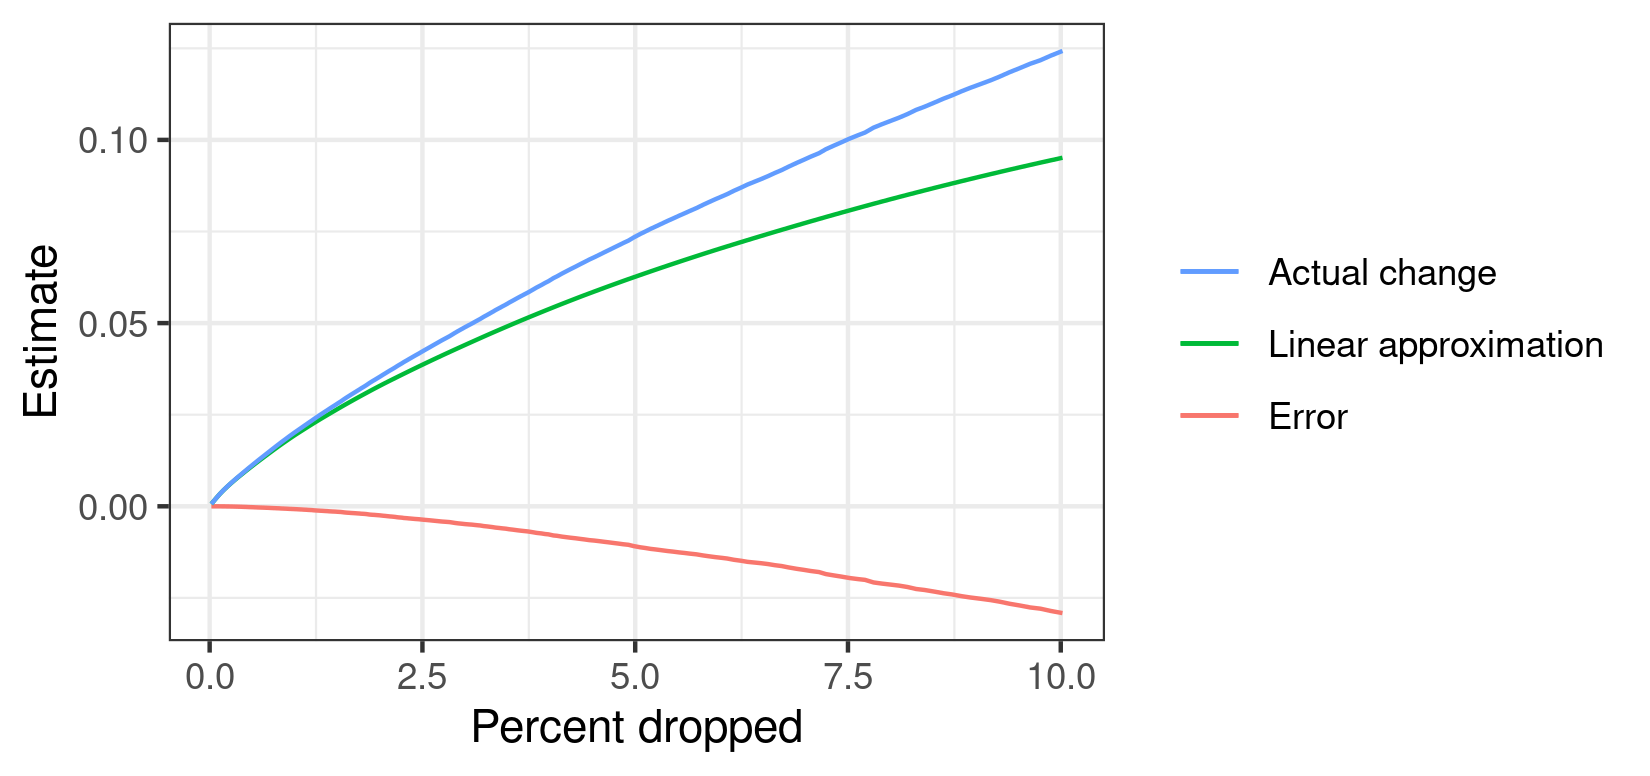
\includegraphics[width=0.98\linewidth,height=0.461\linewidth]{figure/sim-approx-normal-1} 

}

\caption[The actual change, linear approximation to the change, and approximation error.Here, $\sigma_x = \SimAccSigx$, $\sigma_\varepsilon = \SimAccSigeps$, and $\theta_0 = \SimTrueTheta$]{The actual change, linear approximation to the change, and approximation error.Here, $\sigma_x = \SimAccSigx$, $\sigma_\varepsilon = \SimAccSigeps$, and $\theta_0 = \SimTrueTheta$.}\label{fig:sim-approx-normal}
\end{figure}


\end{knitrout}
}

\newcommand{\SimGridNormalGraph}{

\begin{knitrout}
\definecolor{shadecolor}{rgb}{0.969, 0.969, 0.969}\color{fgcolor}\begin{figure}[!h]

{\centering 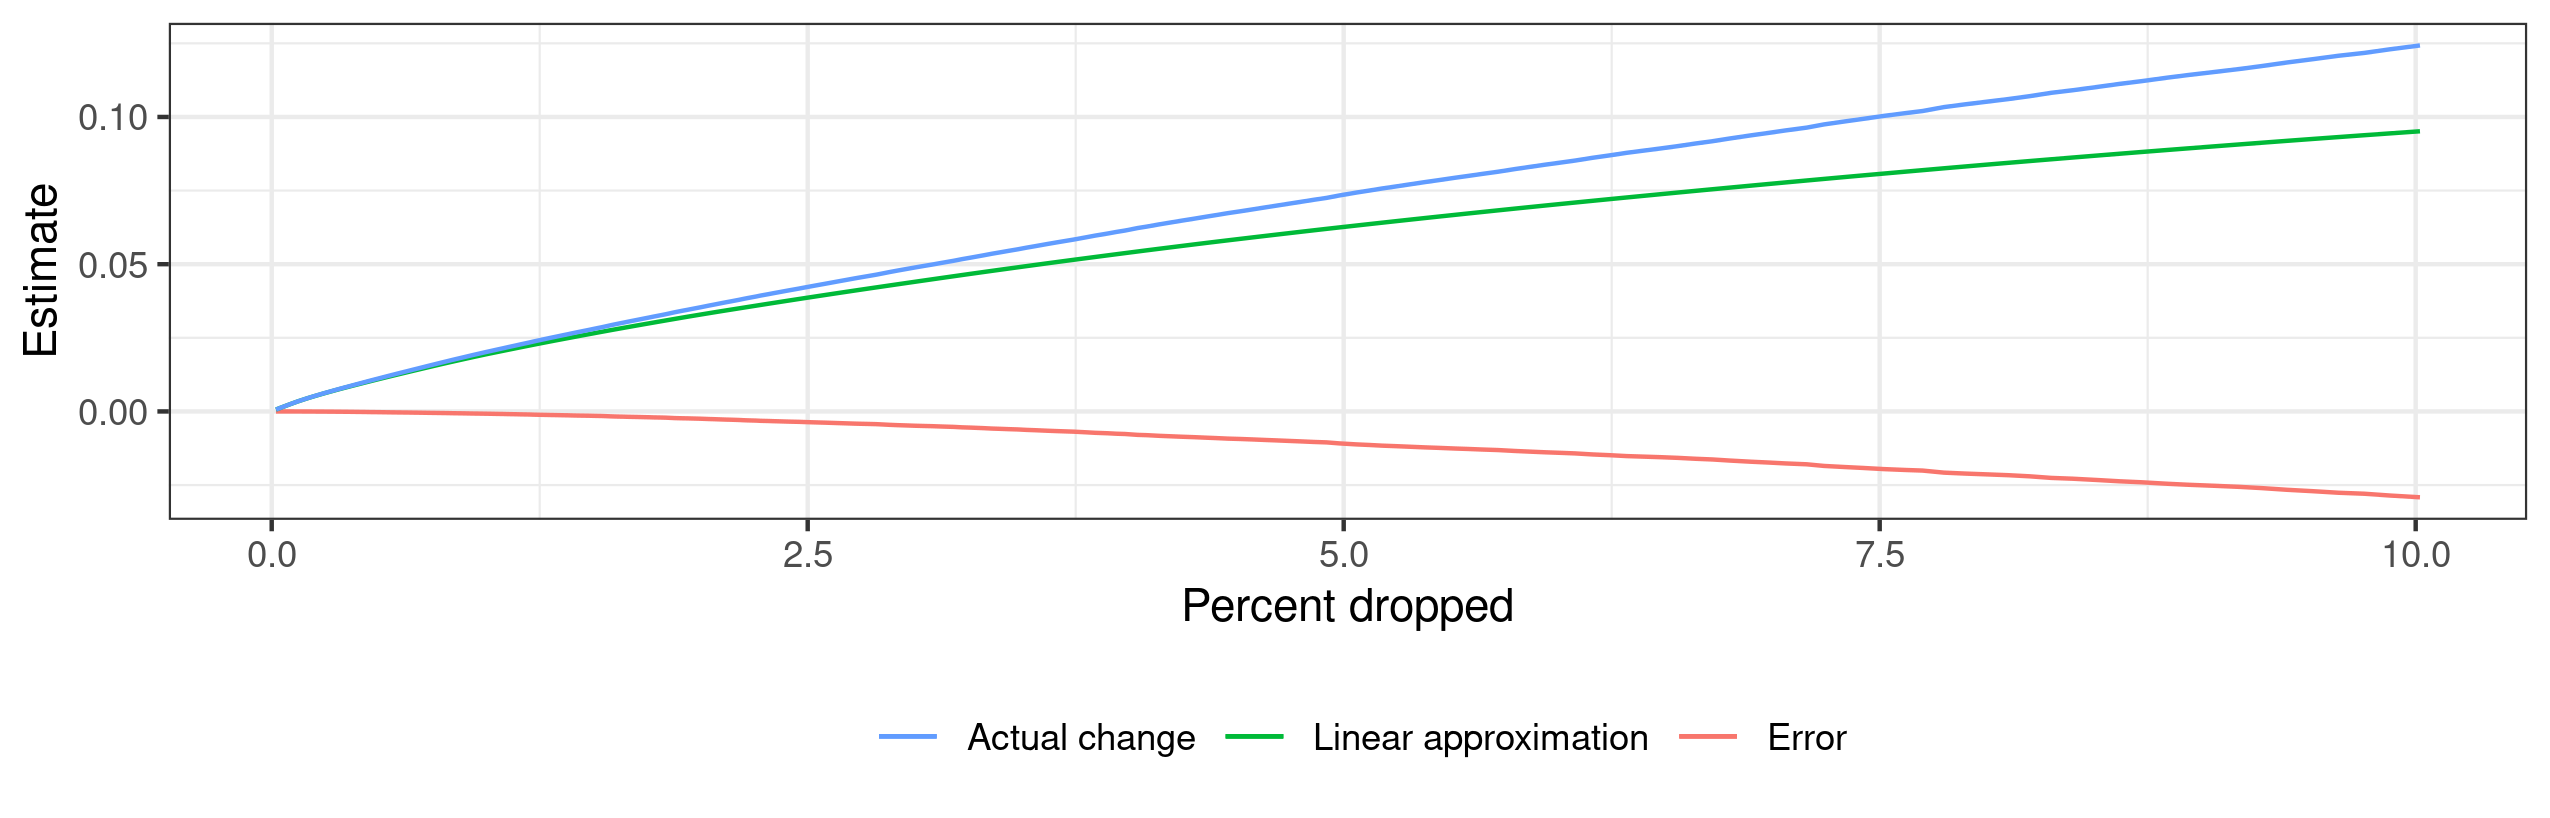
\includegraphics[width=0.98\linewidth,height=0.384\linewidth]{figure/sim-grid-normal-1} 

}

\caption[The approximate perturbation inducing proportion at differing values of $\sigma_x$ and $\sigma_\varepsilon$]{The approximate perturbation inducing proportion at differing values of $\sigma_x$ and $\sigma_\varepsilon$. Red colors indicate datasets whose sign can is predicted to change when dropping less than 1\% of datapoints. The grey areas indicate $\amip{\alpha} = \na$, a failure of the linear approximation to locate any way to change the sign.}\label{fig:sim-grid-normal}
\end{figure}


\end{knitrout}
}
